\documentclass{article}
\usepackage{physics}
\usepackage{graphicx}
\usepackage{caption}
\usepackage{amsmath}
\usepackage{bm}
\usepackage{framed}
\usepackage{authblk}
\usepackage{empheq}
\usepackage{amsfonts}
\usepackage{esint}
\usepackage[makeroom]{cancel}
\usepackage{dsfont}
\usepackage{centernot}
\usepackage{mathtools}
\usepackage{bigints}
\usepackage{amsthm}
\theoremstyle{definition}
\newtheorem{lemma}{Lemma}
\newtheorem{defn}{Definition}[section]
\newtheorem{prop}{Proposition}[section]
\newtheorem{rmk}{Remark}[section]
\newtheorem{thm}{Theorem}[section]
\newtheorem{exmp}{Example}[section]
\newtheorem{prob}{Problem}[section]
\newtheorem{sln}{Solution}[section]
\newtheorem*{prob*}{Problem}
\newtheorem{exer}{Exercise}[section]
\newtheorem*{exer*}{Exercise}
\newtheorem*{sln*}{Solution}
\usepackage{empheq}
\usepackage{tensor}
\usepackage{xcolor}
%\definecolor{colby}{rgb}{0.0, 0.0, 0.5}
\definecolor{MIT}{RGB}{163, 31, 52}
\usepackage[pdftex]{hyperref}
%\hypersetup{colorlinks,urlcolor=colby}
\hypersetup{colorlinks,linkcolor={MIT},citecolor={MIT},urlcolor={MIT}}  
\usepackage[left=1in,right=1in,top=1in,bottom=1in]{geometry}

\usepackage{newpxtext,newpxmath}
\newcommand*\widefbox[1]{\fbox{\hspace{2em}#1\hspace{2em}}}

\newcommand{\p}{\partial}
\newcommand{\R}{\mathbb{R}}
\newcommand{\C}{\mathbb{C}}
\newcommand{\lag}{\mathcal{L}}
\newcommand{\nn}{\nonumber}
\newcommand{\ham}{\mathcal{H}}
\newcommand{\M}{\mathcal{M}}
\newcommand{\I}{\mathcal{I}}
\newcommand{\K}{\mathcal{K}}
\newcommand{\F}{\mathcal{F}}
\newcommand{\w}{\omega}
\newcommand{\lam}{\lambda}
\newcommand{\al}{\alpha}
\newcommand{\be}{\beta}
\newcommand{\x}{\xi}

\newcommand{\G}{\mathcal{G}}

\newcommand{\f}[2]{\frac{#1}{#2}}

\newcommand{\ift}{\infty}

\newcommand{\lp}{\left(}
\newcommand{\rp}{\right)}

\newcommand{\lb}{\left[}
\newcommand{\rb}{\right]}

\newcommand{\lc}{\left\{}
\newcommand{\rc}{\right\}}


\newcommand{\V}{\mathbf{V}}
\newcommand{\U}{\mathcal{U}}
\newcommand{\Id}{\mathcal{I}}
\newcommand{\D}{\mathcal{D}}
\newcommand{\Z}{\mathcal{Z}}

%\setcounter{chapter}{-1}


\usepackage{enumitem}



\usepackage{subfig}
\usepackage{listings}
\captionsetup[lstlisting]{margin=0cm,format=hang,font=small,format=plain,labelfont={bf,up},textfont={it}}
\renewcommand*{\lstlistingname}{Code \textcolor{violet}{\textsl{Mathematica}}}
\definecolor{gris245}{RGB}{245,245,245}
\definecolor{olive}{RGB}{50,140,50}
\definecolor{brun}{RGB}{175,100,80}

%\hypersetup{colorlinks,urlcolor=colby}
\lstset{
	tabsize=4,
	frame=single,
	language=mathematica,
	basicstyle=\scriptsize\ttfamily,
	keywordstyle=\color{black},
	backgroundcolor=\color{gris245},
	commentstyle=\color{gray},
	showstringspaces=false,
	emph={
		r1,
		r2,
		epsilon,epsilon_,
		Newton,Newton_
	},emphstyle={\color{olive}},
	emph={[2]
		L,
		CouleurCourbe,
		PotentielEffectif,
		IdCourbe,
		Courbe
	},emphstyle={[2]\color{blue}},
	emph={[3]r,r_,n,n_},emphstyle={[3]\color{magenta}}
}






\begin{document}
\begin{framed}
\noindent Name: \textbf{Huan Q. Bui}\\
Course: \textbf{8.321 - Quantum Theory I}\\
Problem set: \textbf{\#3}
\end{framed}
	




\noindent \textbf{1. }
\begin{equation*}
A = \begin{pmatrix}
1 & 0 & 1\\
0 & 0 & 0\\
1 & 0 & 1
\end{pmatrix} 
\quad\quad \quad 
B = \begin{pmatrix}
2 & 1 & 1 \\
1 & 0 & -1\\
1 & -1 & 2
\end{pmatrix}.
\end{equation*}

\begin{enumerate}[label=(\alph*)]
	\item To show that $AB$ commute, we simply compute their commutator:
	\begin{align*}
	[A,B] = \begin{pmatrix}
	1 & 0 & 1\\
	0 & 0 & 0\\
	1 & 0 & 1
	\end{pmatrix} 
	\begin{pmatrix}
	2 & 1 & 1 \\
	1 & 0 & -1\\
	1 & -1 & 2
	\end{pmatrix}
	- 
	\begin{pmatrix}
	2 & 1 & 1 \\
	1 & 0 & -1\\
	1 & -1 & 2
	\end{pmatrix}
	\begin{pmatrix}
	1 & 0 & 1\\
	0 & 0 & 0\\
	1 & 0 & 1
	\end{pmatrix} 
	= 
	\begin{pmatrix}
	3 & 0 & 3\\
	0 & 0 & 0\\
	3 & 0 & 3
	\end{pmatrix}
	-
	\begin{pmatrix}
	3 & 0 & 3\\
	0 & 0 & 0\\
	3 & 0 & 3
	\end{pmatrix} = 
	\begin{pmatrix}
	0 & 0 & 0\\
	0 & 0 & 0\\
	0 & 0 & 0
	\end{pmatrix}.   
	\end{align*}
	So, $A$ and $B$ commute.
	
	
	\item Notice that $\rank(A) = 1$. So $A$ must have eigenvalue of zero with multiplicity of two. The other eigenvalue is $2$ by inspection, where the corresponding eigenvector is $(1,0,1)^\top$. The other two $0$-eigenvectors must span the subspace orthogonal to $(1,0,1)^\top$. We may choose $(0,1,0)^\top$ and $(-1,0,1)^\top$.\\
	
	To find the eigenvalues of $B$ we may use the traditional method of characteristic polynomials. 
	\begin{align*}
	0 = \det(B-\lambda \mathbb{I}) = -6-\lambda +4 \lambda^2 - \lambda^3 \implies 0 = (\lambda-3)(\lambda-2)(\lambda+1).
	\end{align*}
	The corresponding eigenvectors are
	\begin{align*}
	&\begin{pmatrix}
	2 & 1 & 1 \\
	1 & 0 & -1\\
	1 & -1 & 2
	\end{pmatrix}\vec{x}_1 = 3\vec{x}_1 \implies \vec{x}_1 = \begin{pmatrix}
	1 \\ 0 \\ 1
	\end{pmatrix}\\
	&\begin{pmatrix}
	2 & 1 & 1 \\
	1 & 0 & -1\\
	1 & -1 & 2
	\end{pmatrix}\vec{x}_2 = 2\vec{x}_2 \implies \vec{x}_2 = \begin{pmatrix}
	-1 \\ -1 \\ 1
	\end{pmatrix}\\
	&\begin{pmatrix}
	2 & 1 & 1 \\
	1 & 0 & -1\\
	1 & -1 & 2
	\end{pmatrix}\vec{x}_3 = -1\vec{x}_3 \implies \vec{x}_3 = \begin{pmatrix}
	-1 \\ 2 \\ 1
	\end{pmatrix}
	\end{align*}
	
	
	\item It is clear that $(1,0,1)^\top$ is a simultaneous eigenvector of $A$ and $B$. Also notice that the eigenvectors $\vec{x}_2$ and $\vec{x}_3$ of $B$ are orthogonal to each other and to $(1,0,1)^\top$. This means $\vec{x}_2$ and $\vec{x}_3$ span the subspace associated with the eigenvalue zero for $A$. Thus, $\vec{x}_2$, $\vec{x}_3$ are eigenvectors of $A$ and it suffices to normalize $\vec{x}_1, \vec{x}_2, \vec{x}_3$ to form a unitary matrix:
	\begin{align*}
	\boxed{U = \begin{pmatrix}
	1/\sqrt{2}  & -1/\sqrt{3} & -1/\sqrt{6}  \\
	0 & -1/\sqrt{3} & 2/\sqrt{6}   \\
	1 /\sqrt{2} & 1/\sqrt{3} & 1/\sqrt{6} 	
	\end{pmatrix}}
	\end{align*} 
	Simultaneous diagonalization of $A$ and $B$:
	\begin{align*}
	&U^\dagger A U = \begin{pmatrix}
	2 & 0 & 0 \\
	0&0&0\\
	0&0&0
	\end{pmatrix}\\
	&U^\dagger B U = \begin{pmatrix}
	3 & 0 & 0 \\
	0 & 2 & 0 \\ 
	0 & 0 & -1
	\end{pmatrix}
	\end{align*}
	as desired.
\end{enumerate}



\noindent \textbf{2. } $N$ spin-$1/2$ particles in 
\begin{align*}
\ham = \ham_2^{(1)} \otimes \ham_2^{(2)} \otimes \dots \otimes \ham_2^{(n)}.
\end{align*}
where each $\ham_2^{(i)}$ is two-dimensional.


\begin{enumerate}[label=(\alph*)]
	\item The dimension of $\ham$ is $2^n$.
	
	\item $S_z = S_z^{(1)} + S_z^{(2)} + \dots + S_z^{(n)}$. There are ${n\choose i}$ product (eigen)states with $i$ particles in $\ket{\uparrow}$ and $(n-i)$ particles in $\ket{\downarrow}$. For the product state with $i$ particles in $\ket{\uparrow}$, the corresponding eigenvalue is 
	\begin{align*}
	\lambda = \f{\hbar}{2}i - \f{\hbar}{2}(n-i) = \f{\hbar}{2}\lp 2i-n \rp,\quad\quad i = 0,1,2,\dots,n
	\end{align*}
	So, the spectrum of $S_z$ is 
	\begin{align*}
	\sigma(S_z) = \lc \f{n\hbar}{2}, \f{(n-2)\hbar}{2},\dots, \f{-(n-2)\hbar}{2}, \f{-n\hbar}{2}   \rc
	\end{align*}
	There are $n+1$ distinct eigenvalues. The multiplicity of each $\lambda_i$ is ${n\choose{i}}$ where $\lambda_i$ is the eigenvalue associated with the product state with $i$ spins in $\ket{\uparrow}$. \\
	
	As a sanity check, the sum of the multiplicities must be $2^n$. This is true due to a well-known combinatorial relation:
	\begin{align*}
	\sum_{i=0}^n {n\choose{i}} = (1+1)^n = 2^n.
	\end{align*}
	
	\item $I = \mathbf{S}^{(1)}\cdot \mathbf{S}^{(2)}+ \mathbf{S}^{(2)}\cdot \mathbf{S}^{(3)} + \dots + \mathbf{S}^{(N-1)}\cdot \mathbf{S}^{(N)}+ \mathbf{S}^{(N)}\cdot \mathbf{S}^{(1)}$. We claim that $[I,S_z] = 0$ and shall prove this by induction. Consider the base case where $N=2$. We may prove it directly by calculating the Kronecker product of the Pauli matrices (working in the $z$-basis).
	\begin{align*}
	&I = \mathbf{S}^{(1)} \cdot \mathbf{S}^{(2)} + \mathbf{S}^{(2)}\cdot \mathbf{S}^{(1)} = 2\lb S_x^{(1)}\otimes S_x^{(2)} + S_y^{(1)} \otimes S_y^{(2)} + S_z^{(1)}\otimes S_z^{(2)}  \rb\\
	&S_z = S_z^{(1)} \otimes \mathbb{I} + \mathbb{I}\otimes S_z^{(2)}.
	\end{align*}
	In Mathematica:
	\begin{lstlisting}
	In[2]:= X = PauliMatrix[1];
	
	In[3]:= Y = PauliMatrix[2];
	
	In[4]:= Z = PauliMatrix[3];
	
	In[6]:= Id = IdentityMatrix[2];
	
	In[8]:= II = 
	2*(KroneckerProduct[X, X] + KroneckerProduct[Y, Y] + 
	KroneckerProduct[Z, Z]);
	
	In[9]:= SZ = KroneckerProduct[Z, Id] + KroneckerProduct[Id, Z];
	
	In[12]:= Commutator = II . SZ - SZ . II;
	
	In[13]:= Commutator
	
	Out[13]= {{0, 0, 0, 0}, {0, 0, 0, 0}, {0, 0, 0, 0}, {0, 0, 0, 0}}
	\end{lstlisting}
	Thus 
	\begin{align*}
	[I^{(2)}, Sz]  = 0.
	\end{align*}
	Now let us assume that $[I, S_z]$ is true up to $N$. We will show that $[I,S_z]$ also holds for $N+1$. This is a straightforward computation. Let us call $I = I_N + I'$ where 
	\begin{align*}
	I_N 
	&= \mathbf{S}^{(1)}\cdot \mathbf{S}^{(2)}+ \mathbf{S}^{(2)}\cdot \mathbf{S}^{(3)} + \dots + \mathbf{S}^{(N-1)}\cdot \mathbf{S}^{(N)}+ \mathbf{S}^{(N)}\cdot \mathbf{S}^{(1)} 
	\end{align*}
	and 
	\begin{align*}
	I' = \mathbf{S}^{(N)}\cdot \mathbf{S}^{(N+1)} + \mathbf{S}^{(N+1)}\cdot \mathbf{S}^{(1)}  -\mathbf{S}^{(N)}\cdot \mathbf{S}^{(1)} 
	\end{align*}
	Moreover, let us write 
	\begin{align*}
	S_z = S_z^{(N+1)} +\sum_{i=1}^N S_z^{(i)}.
	\end{align*}
	Since $I_N$ commute with both $S_z^{N+1}$ (by the fact that $S_z^{N+1}$ does not act on the spins $i=1,\dots,N$) and $\sum_{i=1}^N S_z^{(i)}$ (by inductive hypothesis), we have
	\begin{align*}
	[I,S_z]
	&= \lb I_N + I' , S_z^{(N+1)} +\sum_{i=1}^N S_z^{(i)} \rb \\
	&= \lb I' , S_z^{(N+1)}\rb  +\lb I', \sum_{i=1}^N S_z^{(i)} \rb \\
	&= \lb \mathbf{S}^{(N)}\cdot \mathbf{S}^{(N+1)} + \mathbf{S}^{(N+1)}\cdot \mathbf{S}^{(1)} , S_z^{(N+1)} \rb + \lb \mathbf{S}^{(N)}\cdot \mathbf{S}^{(N+1)} + \mathbf{S}^{(N+1)}\cdot \mathbf{S}^{(1)}  , \sum_{i=1}^N S_z^{(i)}\rb 
	\end{align*}
	where we have used the following facts: 
	\begin{align*}
	&\lb  \mathbf{S}^{(N)}\cdot \mathbf{S}^{(1)} , S_z^{(N+1)} \rb = 0\\
	&\lb \mathbf{S}^{(N)}\cdot \mathbf{S}^{(1)} ,  \sum_{i=1}^N S_z^{(i)} \rb = \lb \mathbf{S}^{(N)}\cdot \mathbf{S}^{(1)}, S_z^{(1)} + S_z^{(N)} \rb = 0
	\end{align*}
	where the second fact comes from the $N=2$ result. We may simplify $[I,S_z]$ even further:
	\begin{align*}
	[I,S_z] 
	&=  \lb \mathbf{S}^{(N)}\cdot \mathbf{S}^{(N+1)} + \mathbf{S}^{(N+1)}\cdot \mathbf{S}^{(1)} , S_z^{(N+1)} \rb + \lb \mathbf{S}^{(N)}\cdot \mathbf{S}^{(N+1)} + \mathbf{S}^{(N+1)}\cdot \mathbf{S}^{(1)}  , S_z^{(1)} + S_z^{(N)}\rb \\
	&= \lb \mathbf{S}^{(N)}\cdot \mathbf{S}^{(N+1)} + \mathbf{S}^{(N+1)}\cdot \mathbf{S}^{(1)} , S_z^{(1)} + S_z^{(N)} + S_z^{(N+1)} \rb\\
	&= \lb \mathbf{S}^{(N)}\cdot \mathbf{S}^{(N+1)}, S_z^{(1)} + S_z^{(N)} + S_z^{(N+1)} \rb + \lb  \mathbf{S}^{(N+1)}\cdot \mathbf{S}^{(1)} ,  S_z^{(1)} + S_z^{(N)} + S_z^{(N+1)}\rb \\
	&= \lb \mathbf{S}^{(N)}\cdot \mathbf{S}^{(N+1)}, S_z^{(N)} + S_z^{(N+1)} \rb + \lb  \mathbf{S}^{(N+1)}\cdot \mathbf{S}^{(1)} ,  S_z^{(1)}  + S_z^{(N+1)}\rb\\
	&= 0 + 0 \\
	&=0 
	\end{align*}
	in view of the $N=2$ base case. We thus conclude that $I$ and $S_z$ are compatible observables.
	 
	
	
	\item Spectrum and degeneracies of $I$ for $N=2,3,4$. 
	\begin{itemize}
		\item $N=2$ :
		\begin{align*}
		\boxed{\sigma(I_2) =  \f{\hbar^2}{4}\times \{ -6, \underbrace{2}_{\text{deg.}=3}  \} }
		\end{align*}
		\item $N=3$:
		\begin{align*}
		\boxed{\sigma(I_3) = \f{\hbar^2}{4}\times \{ \underbrace{-3}_{\text{deg.}=4}, \underbrace{3}_{\text{deg.}=4}  \}} 
		\end{align*}
		\item $N=4$:
		\begin{align*}
		\boxed{\sigma(I_4) = \f{\hbar^2}{4}\times \{ -8, \underbrace{-4}_{\text{deg.}=3}, \underbrace{4}_{\text{deg.}=5}, \underbrace{0}_{\text{deg.}=7}  \} }
		\end{align*}
	\end{itemize}
	For this problem I have worked in units of $\hbar/2 \equiv 1$ and used a brute force via a simple routine in MATLAB which allows me compute the spectrum for large $N$'s. Below is the code. 
	\begin{lstlisting}
	N    = 10;
	state0 = zeros(2^N,1);
	eigv = 0;
	
	Sz = [1 0 ; 0 -1];
	Sx = [0 1 ; 1 0];
	Sy = [0 -complex(0,1); complex(0,1) 0];
	Id = [1 0 ; 0 1];
	
	% ZZ, YY, XX
	cell_ZZ = cell(N,1);
	cell_YY = cell(N,1);
	cell_XX = cell(N,1);
	termZ = zeros(2,2);
	termY = zeros(2,2);
	termX = zeros(2,2);
	operatorsZ = cell(N,1);
	operatorsY = cell(N,1);
	operatorsX = cell(N,1);
	
	for n = 0:N-2
	operatorsZ = horzcat( horzcat( repmat({Id},1,n)  ,horzcat({Sz}, {Sz})), repmat({Id}, 1 , N-2-n));
	operatorsY = horzcat( horzcat( repmat({Id},1,n)  ,horzcat({Sy}, {Sy})), repmat({Id}, 1 , N-2-n));
	operatorsX = horzcat( horzcat( repmat({Id},1,n)  ,horzcat({Sx}, {Sx})), repmat({Id}, 1 , N-2-n));
	termZ = operatorsZ{1};
	termY = operatorsY{1};
	termX = operatorsX{1};
	for o = 2:N 
	termZ = kron(termZ, operatorsZ{o});
	termY = kron(termY, operatorsY{o});
	termX = kron(termX, operatorsX{o});
	end
	cell_ZZ{n+1} = termZ;
	cell_YY{n+1} = termY;
	cell_XX{n+1} = termX;
	end
	
	
	% deals with the periodic term
	operatorsZ = horzcat(horzcat( {Sz}, repmat({Id}, 1, N-2) ), {Sz} );
	operatorsY = horzcat(horzcat( {Sy}, repmat({Id}, 1, N-2) ), {Sy} );
	operatorsX = horzcat(horzcat( {Sx}, repmat({Id}, 1, N-2) ), {Sx} );
	termZ = operatorsZ{1};
	termY = operatorsY{1};
	termX = operatorsX{1};
	for o = 2:N 
	termZ = kron(termZ, operatorsZ{o});
	termY = kron(termY, operatorsY{o});
	termX = kron(termX, operatorsX{o});
	end
	cell_ZZ{N} = termZ;
	cell_YY{N} = termY;
	cell_XX{N} = termX;
	
	% generates Hamiltonian
	Hamiltonian = zeros(2^N,2^N);
	for i = 1:N
	Hamiltonian = Hamiltonian + cell_ZZ{i} + cell_XX{i} + cell_YY{i};
	end
	
	
	[state0, eigv] = eig(Hamiltonian);
	
	disp(transpose(diag(eigv)));
	disp(state0);
	\end{lstlisting}
	
	
	
	\item By running the MATLAB program for a range of $N$'s, we find that
	\begin{align*}
	\boxed{\lambda_\text{max}^{(N)} = N} \quad\quad\text{restoring } \hbar^2/4 \implies \boxed{\lambda_\text{max}^{(N)} = N\hbar^2/4}
	\end{align*}
	with degeneracy $\boxed{N+1}$. Since the degenaracy grows linearly in $N$, we have multiple choices for an eigenvector associated with each of these eigenvalues. However, using MATLAB we may find that the eigenvectors
	\begin{align*}
	\boxed{\ket{\psi} = (0,0,\dots, 1)^\top \quad\quad \text{and} \quad\quad \ket{\phi} = (1,0,\dots,0)^\top} 
	\end{align*}
	are always associated with the largest positive eigenvalue. 
	
	\item The largest $N$ I could compute in a reasonable amount of time (\textbf{48 seconds}) is $\boxed{N=22}$
	\begin{figure}[!htb]
		\centering
		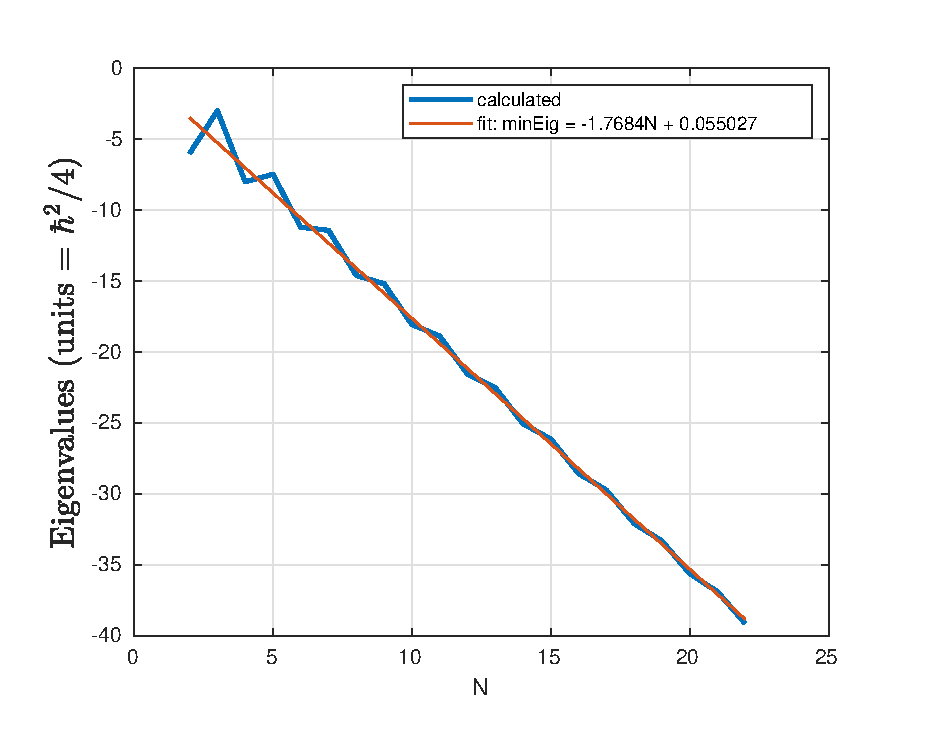
\includegraphics[width=0.75\textwidth]{2f.eps}
	\end{figure}

 
	We see that $\lambda{\text{min}}^{(N)}$ also decreases without bounds and appears to scale linearly in $N$ for small $N$, similar to $\lambda_\text{max}^{(N)}$. I did a linear fit to the data and found that 
	\begin{align*}
	\lambda_\text{min}^{(N)} \approx \f{\hbar^2}{4}\lp -1.7684N + 0.055027\rp .
	\end{align*} 
	A few associated eigenvectors can also be found using the previous MATLAB routine, \textcolor{blue}{but I can't seem to find anything special about these eigenvectors in relation to $N$.}\\
	
	
	
	
	
	MATLAB code (optimized for the minimum eigenvalue problem):
	\begin{lstlisting}
	clear 
	%%%%%%%%%%%%%%%%%%%
	% clock starts
	tic 
	% clock starts
	%%%%%%%%%%%%%%%%%%%
	
	N = 22;
	parfor j=1:N-1
	data(j) = MinEig(j+1);
	end
	plot(2:1:N, data, 'LineWidth',2)
	ylabel('Smallest Eigenvalue')
	xlabel('N')
	grid on
	
	% linear fit
	p = polyfit(2:1:N, data, 1);
	fit = polyval(p,2:1:N);
	hold on
	plot(2:1:N,fit, 'LineWidth', 1)
	hold off
	
	% display fit eqn in legend
	a = p(1);
	b = p(2);
	legend('calculated', ['fit: minEig = ' num2str(a) 'N + ' num2str(b)])
	
	
	
	%%%%%%%%%%%%%%%%%%%
	% clock ends
	Duration = seconds(round(toc));
	Duration.Format = 'hh:mm:ss';
	disp(['Time taken : ' char(Duration)]);
	% disp(['Time in sec: ' num2str(toc)]);
	disp(' ')
	% clock ends
	%%%%%%%%%%%%%%%%%%%
	
	% returns the smallest eigenvalue
	function minEig = MinEig(N)
	
	Sz = sparse([1 0 ; 0 -1]);
	Sx = sparse([0 1 ; 1 0]);
	Sy = sparse([0 -complex(0,1); complex(0,1) 0]);
	Id = sparse([1 0 ; 0 1]);
	
	% ZZ, YY, XX
	cell_ZZ = cell(N,1);
	cell_YY = cell(N,1);
	cell_XX = cell(N,1);
	termZ = zeros(2,2);
	termY = zeros(2,2);
	termX = zeros(2,2);
	operatorsZ = cell(N,1);
	operatorsY = cell(N,1);
	operatorsX = cell(N,1);
	
	parfor n = 0:N-2
	operatorsZ = horzcat( horzcat( repmat({Id},1,n)  ,horzcat({Sz}, {Sz})), repmat({Id}, 1 , N-2-n));
	operatorsY = horzcat( horzcat( repmat({Id},1,n)  ,horzcat({Sy}, {Sy})), repmat({Id}, 1 , N-2-n));
	operatorsX = horzcat( horzcat( repmat({Id},1,n)  ,horzcat({Sx}, {Sx})), repmat({Id}, 1 , N-2-n));
	termZ = operatorsZ{1};
	termY = operatorsY{1};
	termX = operatorsX{1};
	for o = 2:N
	termZ = sparse(kron(termZ, operatorsZ{o}));
	termY = sparse(kron(termY, operatorsY{o}));
	termX = sparse(kron(termX, operatorsX{o}));
	end
	cell_ZZ{n+1} = termZ;
	cell_YY{n+1} = termY;
	cell_XX{n+1} = termX;
	end
	
	% periodic term
	operatorsZ = horzcat(horzcat( {Sz}, repmat({Id}, 1, N-2) ), {Sz} );
	operatorsY = horzcat(horzcat( {Sy}, repmat({Id}, 1, N-2) ), {Sy} );
	operatorsX = horzcat(horzcat( {Sx}, repmat({Id}, 1, N-2) ), {Sx} );
	termZ = operatorsZ{1};
	termY = operatorsY{1};
	termX = operatorsX{1};
	for o = 2:N
	termZ = sparse(kron(termZ, operatorsZ{o}));
	termY = sparse(kron(termY, operatorsY{o}));
	termX = sparse(kron(termX, operatorsX{o}));
	end
	cell_ZZ{N} = termZ;
	cell_YY{N} = termY;
	cell_XX{N} = termX;
	
	% generates Hamiltonian
	Hamiltonian = sparse(2^N,2^N);
	parfor i = 1:N
	Hamiltonian = Hamiltonian + cell_ZZ{i} + cell_XX{i} + cell_YY{i};
	end
	% exact diagonalization
	eigv = eigs(Hamiltonian,1,'smallestreal');
	
	% returns smallest eigenvalue
	minEig = eigv;
	
	end
	\end{lstlisting}
	
	\item We have 
	\begin{align*}
	\ham  = bx S_z -a(1-x)I.
	\end{align*}
	With $b = a\hbar$, we may set $a=1$ and $\hbar=1$, so that 
	\begin{align*}
	\ham = \f{x}{2}S_z - \f{(1-x)}{4}I
	\end{align*}
	where we have nondimensionalized $S_z\propto \hbar/2$ and $I \propto \hbar^2/4$. We can also multiply $\ham$ by $4$ to remove all denominators:
	\begin{align*}
	\ham = 2xS_z - (1-x)I.
	\end{align*}
	
	\begin{figure}[!htb]
		\centering
		\begin{minipage}{0.49\textwidth}
			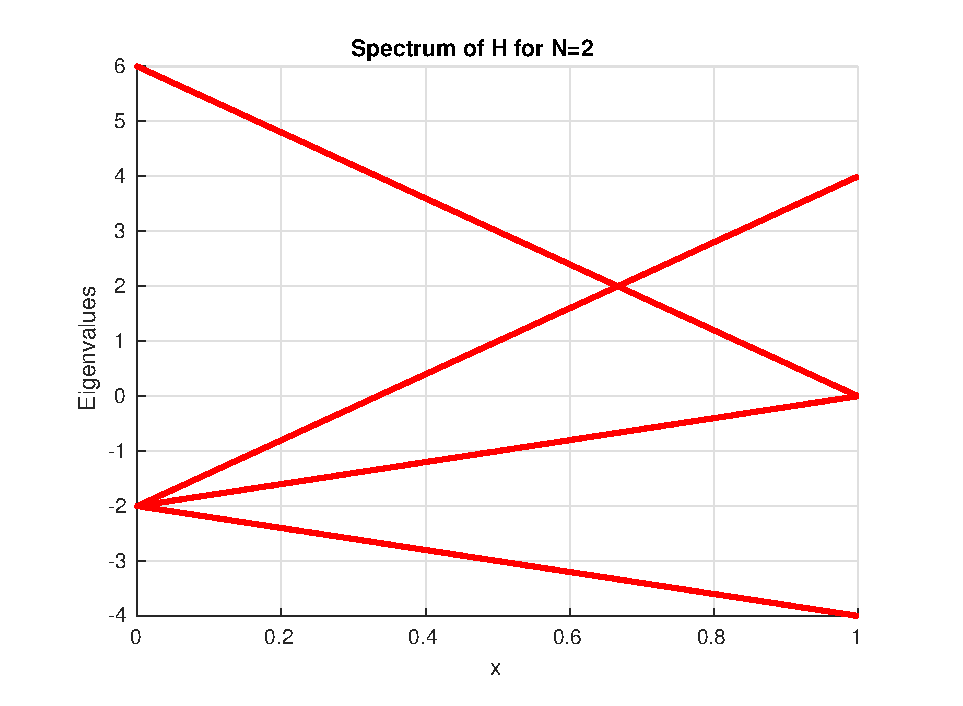
\includegraphics[width=\textwidth]{2g.eps}
		\end{minipage}
		\begin{minipage}{0.49\textwidth}
			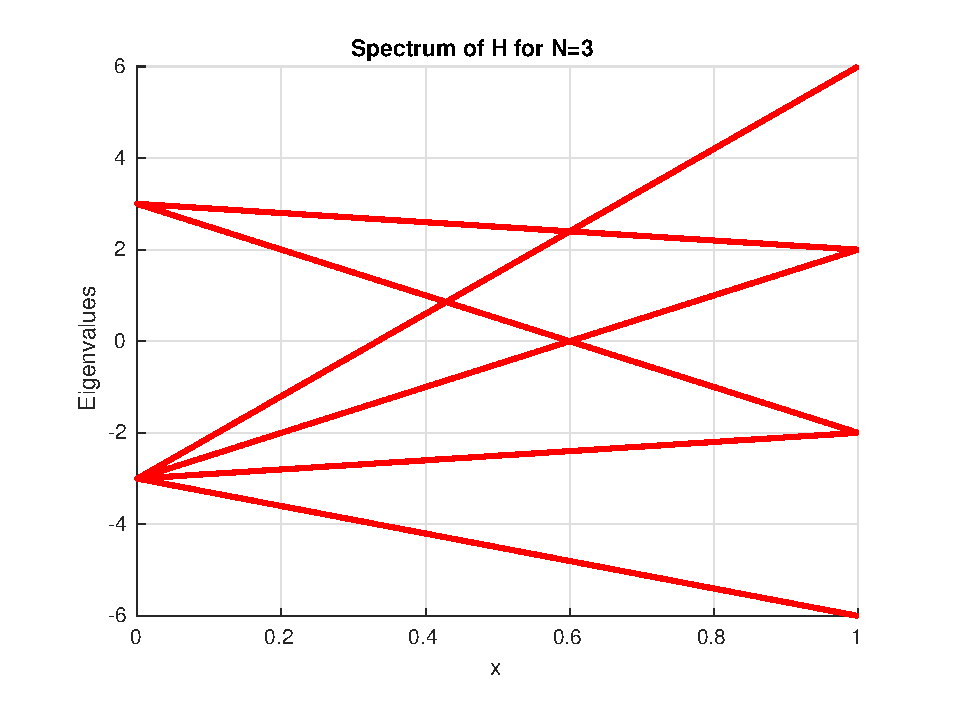
\includegraphics[width=\textwidth]{2g_N3.eps}
		\end{minipage}
		\begin{minipage}{0.49\textwidth}
			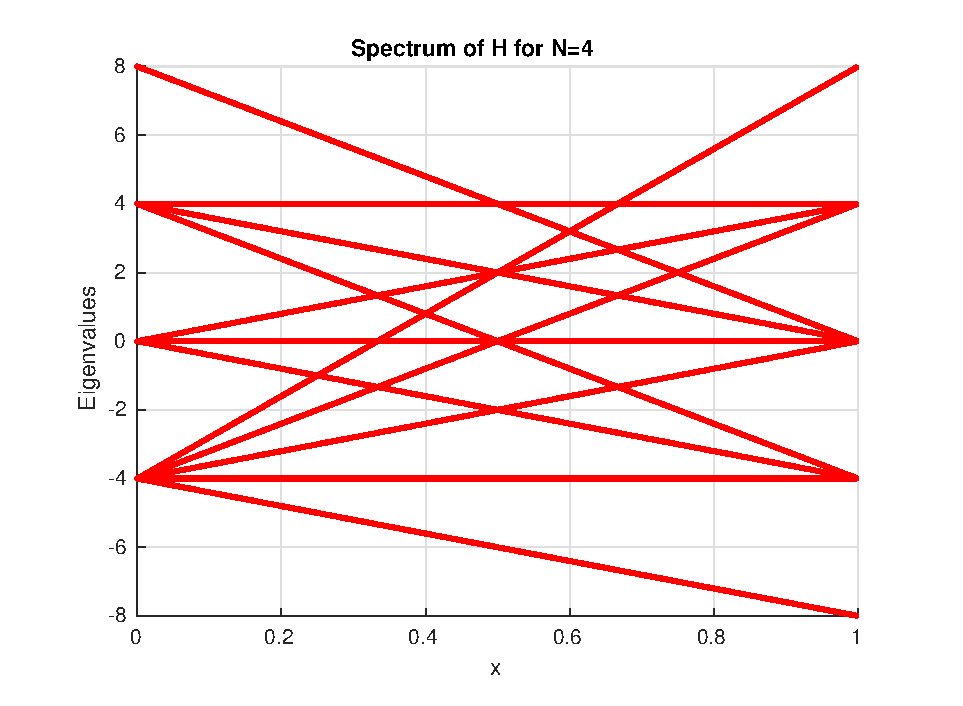
\includegraphics[width=\textwidth]{2g_N4.eps}
		\end{minipage}
	\end{figure}

	The figures generated using the MATLAB code below show good agreement with what we found in the previous parts (setting $x=0$ and flipping the signs of the spectrum gives the results of Part (d)). When $x=1$, the spectra of $H$ are twice what we found in Part (b), which can be explained by the extra leading factor of $2$ on $S_z$ in the Hamiltonian, but are otherwise consistent. For example, at $x=1$ and $N=3$ we find $4=3+1$ distinct eigenvalues. To count degeneracies requires looking at the spectra numerically, since some of the splittings in the figures overlap. But in any case, the degeneracies are also consistent with what we found in Part (b). 
	\begin{lstlisting}
	clear crc
	clear all
	
	N = 4;
	res = 400;
	x = 0:1/res:1-1/res;
	figure(1)
	for j=0:1:res-1
	eigv = Bfield(N,j/res); 
	hold on
	X = (j/res)*ones(2^N,1);
	plot(X,eigv,'Marker','o', 'MarkerSize', 2, 'Color', 'r', 'LineStyle', 'None')
	hold off
	end
	hold off
	grid on
	
	xlabel('$x$', 'Interpreter', 'latex', 'FontSize', 16)
	ylabel('Eigenvalues (units = $\hbar^2/4$)', 'Interpreter','latex', 'FontSize', 16)
	title(['Spectrum of H for N=' num2str(N)])
	
	
	
	
	function eigv = Bfield(N,x)
	Sz = [1 0 ; 0 -1];
	Sx = [0 1 ; 1 0];
	Sy = [0 -complex(0,1); complex(0,1) 0];
	Id = [1 0 ; 0 1];
	
	% ZZ, YY, XX
	cell_ZZ = cell(N,1);
	cell_YY = cell(N,1);
	cell_XX = cell(N,1);
	termZ = zeros(2,2);
	termY = zeros(2,2);
	termX = zeros(2,2);
	operatorsZ = cell(N,1);
	operatorsY = cell(N,1);
	operatorsX = cell(N,1);
	
	for n = 0:N-2
	operatorsZ = horzcat( horzcat( repmat({Id},1,n)  ,horzcat({Sz}, {Sz})), repmat({Id}, 1 , N-2-n));
	operatorsY = horzcat( horzcat( repmat({Id},1,n)  ,horzcat({Sy}, {Sy})), repmat({Id}, 1 , N-2-n));
	operatorsX = horzcat( horzcat( repmat({Id},1,n)  ,horzcat({Sx}, {Sx})), repmat({Id}, 1 , N-2-n));
	termZ = operatorsZ{1};
	termY = operatorsY{1};
	termX = operatorsX{1};
	for o = 2:N 
	termZ = kron(termZ, operatorsZ{o});
	termY = kron(termY, operatorsY{o});
	termX = kron(termX, operatorsX{o});
	end
	cell_ZZ{n+1} = termZ;
	cell_YY{n+1} = termY;
	cell_XX{n+1} = termX;
	end
	
	
	% deals with the periodic term
	operatorsZ = horzcat(horzcat( {Sz}, repmat({Id}, 1, N-2) ), {Sz} );
	operatorsY = horzcat(horzcat( {Sy}, repmat({Id}, 1, N-2) ), {Sy} );
	operatorsX = horzcat(horzcat( {Sx}, repmat({Id}, 1, N-2) ), {Sx} );
	termZ = operatorsZ{1};
	termY = operatorsY{1};
	termX = operatorsX{1};
	for o = 2:N 
	termZ = kron(termZ, operatorsZ{o});
	termY = kron(termY, operatorsY{o});
	termX = kron(termX, operatorsX{o});
	end
	cell_ZZ{N} = termZ;
	cell_YY{N} = termY;
	cell_XX{N} = termX;
	
	
	% generates Sz
	% generate the fZ cell array of the Hamiltonian:
	term = sparse(2,2);
	cell_fZ = cell(N,1);
	operators = cell(N,1);
	for n = 0:N-1
	operators = horzcat( horzcat( repmat({Id},1,n), {Sz}), repmat({Id}, 1 , N-1-n));
	term = operators{1};
	for o = 2:N 
	term = sparse(kron(term, operators{o}));
	end
	cell_fZ{n+1} = term;
	end
	
	% generates Hamiltonian
	Hamiltonian = zeros(2^N,2^N);
	for i = 1:N
	Hamiltonian = Hamiltonian + 2*x*cell_fZ{i} - (1-x)*(cell_ZZ{i} + cell_XX{i} + cell_YY{i});
	end
	
	eigv = eig(Hamiltonian);
	
	end

	\end{lstlisting}
\end{enumerate}






\noindent \textbf{3. Qubits.} We have a system of $4$ spins in $\ket{+,x}$. We shall proceed with this problem by brute force, at least for the first two parts. 


\begin{enumerate}[label=(\alph*)]
	\item In Mathematica, we may work in the $z$-basis and explicitly compute 
	\begin{align*}
	\mathbb{I}\otimes \mathbb{I} \otimes (\mathbf{S}^{(3)}\cdot \mathbf{S}^{(4)})
	\end{align*}
	as well as its spectrum $\{ -3\hbar^2/4, \hbar^2/4 \}$ and eigenvectors, using Mathematica. Using the formula 
	\begin{align*}
	\Pr(A=a) = \sum_{j:a_j=a} \abs{\bra{a_j} \ket{\al}}^2,
	\end{align*}
	for the input state $\ket{\al} = \ket{++++}$, we find 
	\begin{align*}
	\boxed{\Pr(-3\hbar^2/4) = 0} \quad\quad \boxed{\Pr(\hbar^2/4) = 1}
	\end{align*}
	
	
	
	
	
	
	\begin{lstlisting}
	In[1]:= X = PauliMatrix[1];
	
	In[2]:= Y = PauliMatrix[2];
	
	In[3]:= Z = PauliMatrix[3];
	
	In[4]:= Id = IdentityMatrix[2];
	
	In[5]:= T[x_, y_] := KroneckerProduct[x, y];
	
	In[60]:= S34 = (h^2/4)*(T[Id, T[Id, T[X, X] + T[Y, Y] + T[Z, Z]]]);
	
	In[61]:= Eigenvalues[S34]
	
	Out[61]= {-((3 h^2)/4), -((3 h^2)/4), -((3 h^2)/4), -((3 h^2)/
	4), h^2/4, h^2/4, h^2/4, h^2/4, h^2/4, h^2/4, h^2/4, h^2/4, h^2/4, \
	h^2/4, h^2/4, h^2/4}
	
	In[89]:= E34 = Eigenvectors[S34];
	
	In[64]:= XPlus = (1/Sqrt[2])*{{1}, {1}};
	
	In[65]:= XMinus = (1/Sqrt[2])*{{1}, {-1}};
	
	In[68]:= PPPP = T[XPlus, T[XPlus, T[XPlus, XPlus]]];
	
	In[80]:= (*Part (a)*)
	
	In[74]:= (*Eigv -3h^2/4*)
	
	In[77]:= Dot[Conjugate[E34[[1]]/Norm[E34[[1]]]], PPPP]^2 + 
	Dot[Conjugate[E34[[2]]/Norm[E34[[2]]]], PPPP]^2 +
	Dot[Conjugate[E34[[3]]/Norm[E34[[3]]]], PPPP]^2 +
	Dot[Conjugate[E34[[4]]/Norm[E34[[4]]]], PPPP]^2
	
	Out[77]= {0}
	
	In[79]:= (*Eigv h^2/4*)
	
	In[78]:= Sum[
	Dot[Conjugate[E34[[i]]]/Norm[E34[[i]]], PPPP]^2, {i, 5, 16}]
	
	Out[78]= {1}
	\end{lstlisting}
	
	
	
	\item Measuring $S_z^{(3)}$ $\ket{++++}$ gives $\hbar/2$ and $-\hbar/2$ with equal probability ($1/2$). The state after this measurement is $\ket{++\uparrow +}$ or $\ket{++\downarrow +}$. Now we measure $\mathbf{S}^{(3)}\cdot \mathbf{S}^{(4)}$. From the previous part we know that there are only two eigenspaces associated with the distinct eigenvalues $-3\hbar^2/4$ and $\hbar^2/4$. So, we construct two projection operators $P_1$ and $P_2$:
	\begin{align*}
	P_1 = \sum_{i=1}^4 \ket{ \epsilon^{(34)}_i} \bra{\epsilon^{(34)}_i} \quad\quad \text{and}\quad\quad P_2 = \sum_{i=5}^{16} \ket{ \epsilon^{(34)}_i} \bra{\epsilon^{(34)}_i}
	\end{align*}
	where $\ket{ \epsilon^{(34)}_i}$ for $i=1,\dots,4$ are the $-3\hbar^2/4$-eigenstates and $\ket{ \epsilon^{(34)}_i}$ for $i=5,\dots,16$ are the $\hbar^2/4$-eigenstates. With this, we can now compute the probabilities for each possible outcome:
	\begin{align*}
	&\Pr\lp \f{\hbar}{2} \to \f{-3\hbar^2}{4} \rp = \f{1}{2} \bra{++\uparrow +} P_1 \ket{++\uparrow +} = \f{1}{2}\f{1}{4} = \f{1}{8} \\
	&\Pr\lp \f{\hbar}{2} \to \f{\hbar^2}{4} \rp =  \f{1}{2} \bra{++\uparrow +} P_2 \ket{++\uparrow +} = \f{1}{2}\f{3}{4} = \f{3}{8}\\
	&\Pr\lp \f{-\hbar}{2} \to \f{\hbar^2}{4} \rp =  \f{1}{2} \bra{++\downarrow +} P_1 \ket{++\downarrow +} = \f{1}{2}\f{1}{4} = \f{1}{8}\\
	&\Pr\lp \f{-\hbar}{2} \to \f{-3\hbar^2}{4} \rp =  \f{1}{2} \bra{++\downarrow +} P_2 \ket{++\downarrow +} = \f{1}{2}\f{3}{4} = \f{3}{8}
	\end{align*}
	Thus, the total probabilities after the $\mathbf{S}^{(3)}\cdot \mathbf{S^{(4)}}$ measurement are 
	\begin{align*}
	\boxed{\Pr\lp \f{-3\hbar^2}{4} \rp = \f{1}{8} + \f{1}{8} = {\f{1}{4}}} \quad\quad 
	\boxed{\Pr\lp \f{\hbar^2}{4} \rp = \f{3}{4}}
	\end{align*}
	Mathematica code:
	\begin{lstlisting}
	In[18]:= (*Part (b)*)
	
	In[66]:= PPUP = Flatten[T[XPlus, T[XPlus, T[{1, 0}, XPlus]]]];
	
	In[65]:= PPDP = Flatten[T[XPlus, T[XPlus, T[{0, 1}, XPlus]]]];
	
	In[67]:= P1 = 
	Sum[Outer[Times, E34[[i]]/Norm[E34[[i]]], 
	E34[[i]]/Norm[E34[[i]] ]], {i, 1, 4}] ;
	
	In[68]:= P2 = 
	Sum[Outer[Times, E34[[i]]/Norm[E34[[i]]], 
	E34[[i]]/Norm[E34[[i]] ]], {i, 5, 16}] ;
	
	In[73]:= Dot[PPDP/Norm[PPDP], P2 . PPDP/Norm[PPDP]]
	
	Out[73]= 3/4
	
	In[70]:= Dot[PPDP/Norm[PPDP], P1 . PPDP/Norm[PPDP]](*-3h^2/4*)
	
	Out[70]= 1/4
	
	In[71]:= Dot[PPUP/Norm[PPUP], P2 . PPUP/Norm[PPUP]]
	
	Out[71]= 3/4
	
	In[72]:= Dot[PPUP/Norm[PPUP], P1 . PPUP/Norm[PPUP]](*-3h^2/4*)
	
	Out[72]= 1/4
	\end{lstlisting}
	
	
	
	\item This is very similar to Part (b), except that we have to take an extra step after measuring $\mathbf{S}^{(2)}\cdot \mathbf{S}^{(3)}$. In view of Part (b), we already have
	\begin{align*}
	&\Pr\lp \f{\hbar}{2} \to \f{-3\hbar^2}{4} \rp = \f{1}{2} \bra{++\uparrow +} P_1 \ket{++\uparrow +} = \f{1}{2}\f{1}{4} = \f{1}{8} \\
	&\Pr\lp \f{\hbar}{2} \to \f{\hbar^2}{4} \rp =  \f{1}{2} \bra{++\uparrow +} P_2 \ket{++\uparrow +} = \f{1}{2}\f{3}{4} = \f{3}{8}\\
	&\Pr\lp \f{-\hbar}{2} \to \f{\hbar^2}{4} \rp =  \f{1}{2} \bra{++\downarrow +} P_1 \ket{++\downarrow +} = \f{1}{2}\f{1}{4} = \f{1}{8}\\
	&\Pr\lp \f{-\hbar}{2} \to \f{-3\hbar^2}{4} \rp =  \f{1}{2} \bra{++\downarrow +} P_2 \ket{++\downarrow +} = \f{1}{2}\f{3}{4} = \f{3}{8}
	\end{align*}
	After the first two meausurements. In order to find what the probabilities are when we measure $\mathbf{S}^{(3)}\cdot \mathbf{S}^{(4)}$, we must find out what the state is after the first two measurements. We know that after measuring $S_z^{(2)}$, we will end up with $\ket{+\uparrow ++}$ or $\ket{+ \downarrow ++}$. Let the projection operators $P_{1c}$ and $P_{2c}$ be defined similar to $P_1$ and $P_2$ in Part (b) but for $\mathbf{S}^{(2)} \cdot \mathbf{S}^{(3)}$, we find four possible outcomes after the first two measurements:
	\begin{align*}
	&\f{\hbar}{2} \to \f{-3\hbar^2}{4}: \quad\ket{\psi_{1c}} = \f{P_{1c} \ket{+\uparrow ++}}{\norm{P_{1c} \ket{+\uparrow ++}}}\\
	&\f{\hbar}{2} \to \f{\hbar^2}{4}: \quad\ket{\psi_{2c}} = \f{P_{2c} \ket{+\uparrow ++}}{\norm{P_{2c} \ket{+\uparrow ++}}}\\
	&\f{-\hbar}{2} \to \f{-3\hbar^2}{4}: \quad\ket{\psi_{3c}} = \f{P_{1c} \ket{+\downarrow ++}}{\norm{P_{1c} \ket{+\downarrow ++}}}\\
	&\f{-\hbar}{2} \to \f{\hbar^2}{4}: \quad\ket{\psi_{4c}} = \f{P_{2c} \ket{+\downarrow ++}}{\norm{P_{2c} \ket{+\downarrow ++}}}
	\end{align*}
	Now it remains to compute $\bra{\psi_i} P_1 \ket{\psi_i}$ to find the probabilities of measuring $-3\hbar^2/4$ and $\hbar^2/4$ after the third measurement $\mathbf{S}^{(3)}\cdot \mathbf{S}^{(4)}$. It turns out that there are symmetries to the outcome, so we will write the outcomes compactly as 
	\begin{align*}
	&\Pr\lp \pm \f{\hbar}{2} \to \f{-3\hbar^2}{4} \to \f{-3\hbar^2}{4}\rp = \f{1}{2}\f{1}{4}\f{1}{4} = \f{1}{32}\\
	&\Pr\lp \pm \f{\hbar}{2} \to \f{-3\hbar^2}{4} \to \f{\hbar^2}{4}\rp = \f{1}{2}\f{1}{4}\f{3}{4} = \f{3}{32}\\
	&\Pr\lp \pm \f{\hbar}{2} \to \f{\hbar^2}{4} \to \f{-3\hbar^2}{4}\rp = \f{1}{2}\f{3}{4}\f{1}{12} = \f{1}{32} \\
	&\Pr\lp \pm \f{\hbar}{2} \to \f{\hbar^2}{4} \to \f{\hbar^2}{4}\rp = \f{1}{2}\f{3}{4}\f{11}{12} = \f{11}{32} 
	\end{align*}
	Here, $\pm$ is used in the sense of ``XOR.'' Thus, the sum of the probabilities above is $1/2$  rather than $1$. The missing factor of $2$ can be put back by adding the contributions from both branches $\hbar/2$ and $-\hbar/2$ from the first measurement.\\
	
	The total probabilities after the $\mathbf{S}^{(3)}\cdot \mathbf{S^{(4)}}$ measurement are 
	\begin{align*}
	\boxed{\Pr \lp \f{-3\hbar^2}{4} \rp = 2\lp \f{1}{32} + \f{1}{32}\rp = \f{1}{8}} \quad\quad 
	\boxed{\Pr \lp \f{\hbar^2}{4} \rp = \f{7}{8}} 
	\end{align*}	
	Mathematica code:
	\begin{lstlisting}
	In[27]:= (*Part (c)*)
	
	In[28]:= S23 = (h^2/4)*(T[Id, T[T[X, X] + T[Y, Y] + T[Z, Z], Id]]);
	
	In[29]:= PUPP = Flatten[T[XPlus, T[{1, 0}, T[XPlus, XPlus]]]];
	
	In[30]:= PDPP = Flatten[T[XPlus, T[{0, 1}, T[XPlus, XPlus]]]];
	
	In[74]:= Eigenvalues[S23];
	
	In[32]:= E23 = Eigenvectors[S23];
	
	In[33]:= P1c = 
	Sum[Outer[Times, E23[[i]]/Norm[E23[[i]]], 
	E23[[i]]/Norm[E23[[i]] ]], {i, 1, 4}] ;
	
	In[34]:= P2c = 
	Sum[Outer[Times, E23[[i]]/Norm[E23[[i]]], 
	E23[[i]]/Norm[E23[[i]] ]], {i, 5, 16}] ;
	
	In[36]:= Dot[PDPP/Norm[PDPP], P2c . PDPP/Norm[PDPP]](*h^2/4*);
	
	In[38]:= v1c = P2c . PDPP/Norm[P2c . PDPP];
	
	In[41]:= Dot[PDPP/Norm[PDPP], P1c . PDPP/Norm[PDPP]](*-3h^2/4*);
	
	In[43]:= v2c = P1c . PDPP/Norm[P1c . PDPP];
	
	In[46]:= Dot[PUPP/Norm[PUPP], P2c . PUPP/Norm[PUPP]](*h^2/4*);
	
	In[48]:= v3c = P2c . PUPP/Norm[P2c . PUPP];
	
	In[51]:= Dot[PUPP/Norm[PUPP], P1c . PUPP/Norm[PUPP]](*-3h^2/4*);
	
	In[53]:= v4c = P1c . PUPP/Norm[P1c . PUPP];
	
	In[56]:= Dot[v1c, P1 . v1c]
	
	Out[56]= 1/12
	
	In[57]:= Dot[v2c, P1 . v2c]
	
	Out[57]= 1/4
	
	In[58]:= Dot[v3c, P1 . v3c]
	
	Out[58]= 1/12
	
	In[59]:= Dot[v4c, P1 . v4c]
	
	Out[59]= 1/4
	\end{lstlisting}
	
	
	
	\item This is similar to Part (c), except that we need to take an extra step for another $\mathbf{S}\cdot \mathbf{S}$ measurement. To do this, let us find the probability of measuring $-3\hbar^2/4$ in the end. All the possible paths to get to this value are
	\begin{align*}
	\pm \f{\hbar}{2} \to \lp \f{-3\hbar^2}{4} \text{ or } \f{\hbar^2}{4} \rp \to \lp \f{-3\hbar^2}{4} \text{ or } \f{\hbar^2}{4} \rp \to \f{-3\hbar^2}{4}.
	\end{align*}
	We need to compute four values in Mathematica (where $\pm$ is once again used in the sense of XOR):
	\begin{align*}
	&\Pr\lp \f{\pm \hbar}{2}\to \f{\hbar^2}{4}\to \f{\hbar^2}{4} \to \f{-3\hbar^2}{4} \rp = \f{1}{2}\f{3}{4}\f{11}{12}\f{1}{44} = \f{1}{128} \\
	&\Pr\lp \f{\pm \hbar}{2}\to \f{\hbar^2}{4}\to \f{-3\hbar^2}{4} \to \f{-3\hbar^2}{4} \rp = \f{1}{2}\f{3}{4}\f{1}{12}\f{1}{4} = \f{1}{128} \\
	&\Pr\lp \f{\pm \hbar}{2}\to \f{-3\hbar^2}{4}\to \f{\hbar^2}{4} \to \f{-3\hbar^2}{4} \rp = 
	\f{1}{2}\f{1}{4}\f{3}{4}\f{1}{12} = \f{1}{128} \\
	&\Pr\lp \f{\pm \hbar}{2}\to \f{-3\hbar^2}{4}\to \f{-3\hbar^2}{4} \to \f{-3\hbar^2}{4} \rp =
	\f{1}{2}\f{1}{4}\f{1}{4}\f{1}{4}  = \f{1}{128}
	\end{align*}
	Corresponding to each sequence above is one which ends in $\hbar^2/4$, with the following probabilities:
	\begin{align*}
	&\Pr\lp \f{\pm \hbar}{2}\to \f{\hbar^2}{4}\to \f{\hbar^2}{4} \to \f{\hbar^2}{4} \rp = \f{1}{2}\f{3}{4}\f{11}{12}\f{43}{44} = \f{43}{128}\\
	&\Pr\lp \f{\pm \hbar}{2}\to \f{\hbar^2}{4}\to \f{-3\hbar^2}{4} \to \f{\hbar^2}{4} \rp = \f{1}{2}\f{3}{4}\f{1}{12}\f{3}{4} = \f{3}{128} \\
	&\Pr\lp \f{\pm \hbar}{2}\to \f{-3\hbar^2}{4}\to \f{\hbar^2}{4} \to \f{\hbar^2}{4} \rp = 
	\f{1}{2}\f{1}{4}\f{3}{4}\f{11}{12} =  \f{11}{128}\\
	&\Pr\lp \f{\pm \hbar}{2}\to \f{-3\hbar^2}{4}\to \f{-3\hbar^2}{4} \to \f{\hbar^2}{4} \rp =
	\f{1}{2}\f{1}{4}\f{1}{4}\f{3}{4} = \f{3}{128}
	\end{align*}
	With these, we can find 
	\begin{align*}
	\boxed{\Pr \lp  \f{-3\hbar^2}{4} \rp = 2\times \f{1+1+1+1}{128} = \f{1}{16}} \quad\quad \boxed{\Pr\lp \f{\hbar^2}{4} \rp = \f{15}{16}}
	\end{align*}
	Mathematica code:
	\begin{lstlisting}
	In[61]:= (*Part (d)*)
	
	In[75]:= S12 = (h^2/4)*(T[T[T[X, X] + T[Y, Y] + T[Z, Z], Id], Id]);
	
	In[77]:= UPPP = Flatten[T[{1, 0}, T[XPlus, T[XPlus, XPlus]]]];
	
	In[78]:= DPPP = Flatten[T[{0, 1}, T[XPlus, T[XPlus, XPlus]]]];
	
	In[80]:= E12 = Eigenvectors[S12];
	
	In[81]:= P1d = 
	Sum[Outer[Times, E12[[i]]/Norm[E12[[i]]], 
	E12[[i]]/Norm[E12[[i]] ]], {i, 1, 4}] ;
	
	In[82]:= P2d = 
	Sum[Outer[Times, E12[[i]]/Norm[E12[[i]]], 
	E12[[i]]/Norm[E12[[i]] ]], {i, 5, 16}] ;
	
	(*h/2 --> -3h^2/4*)
	
	In[86]:= v1 = P1d . UPPP/Norm[P1d . UPPP];
	
	(*h/2 --> -3h^2/4 --> -3h^2/4*)
	
	In[87]:= v2 = P1c . v1/Norm[P1c . v1];
	
	(*h/2 --> -3h^2/4 --> -3h^2/4 --> -3h^2/4*)
	
	In[92]:= Dot[v2, P1 . v2]
	
	Out[92]= 1/4
	
	(*h/2 --> -3h^2/4 --> h^2/4*)
	
	In[100]:= v3 = P2c . v1/Norm[P2c . v1];
	
	(*h/2 --> -3h^2/4 --> h^2/4 --> -3h^2/4*)
	
	In[101]:= Dot[v3, P1 . v3]
	
	Out[101]= 1/12
	
	(*h/2 --> h^2/4*)
	
	In[104]:= v4 = P2d . UPPP/Norm[P2d . UPPP];
	
	(*h/2 --> h^2/4 --> -3h^2/4*)
	
	In[106]:= v5 = P1c . v4/Norm[P1c . v4];
	
	(*h/2 --> h^2/4 --> -3h^2/4 --> -3h^2/4*)
	
	In[108]:= Dot[v5, P1 . v5]
	
	Out[108]= 1/4
	
	(*h/2 --> h^2/4 --> h^2/4*)
	
	In[111]:= v6 = P2c . v4/Norm[P2c . v4];
	
	In[112]:= Dot[v6, P1 . v6]
	
	Out[112]= 1/44
	\end{lstlisting}
	
	
	\item We  notice that the previous two measurements $S_z^{(1)}$ and $\mathbf{S}^{(1)}\cdot \mathbf{S}^{(2)}$ do not affect the states of spins 3 and 4. This means that after the first two measurements, we have the same result as Part (b) but for spins 1 and 2. 
	\begin{align*}
	&\Pr\lp \f{\hbar}{2} \to \f{-3\hbar^2}{4} \rp = \f{1}{2} \bra{\uparrow +++} P_{1e} \ket{\uparrow +++} = \f{1}{2}\f{1}{4} = \f{1}{8} \\
	&\Pr\lp \f{\hbar}{2} \to \f{\hbar^2}{4} \rp =  \f{1}{2} \bra{\uparrow +++} P_{2e} \ket{\uparrow +++} = \f{1}{2}\f{3}{4} = \f{3}{8}\\
	&\Pr\lp \f{-\hbar}{2} \to \f{\hbar^2}{4} \rp =  \f{1}{2} \bra{\downarrow +++} P_{1e} \ket{\downarrow +++} = \f{1}{2}\f{1}{4} = \f{1}{8}\\
	&\Pr\lp \f{-\hbar}{2} \to \f{-3\hbar^2}{4} \rp =  \f{1}{2} \bra{\downarrow +++} P_{2e} \ket{\downarrow +++} = \f{1}{2}\f{3}{4} = \f{3}{8}
	\end{align*}
	Since the $\mathbf{S}^{(3)}\cdot \mathbf{S}^{(4)}$ measurement has nothing to do with spins 1 and 2, the outcomes and probabilities of this measurement is the same as that for Part (a):
	\begin{align*}
	\boxed{\Pr\lp \f{-3\hbar^2}{4} \rp = 0} \quad\quad \boxed{\Pr\lp \f{\hbar^2}{4} \rp = 1}
	\end{align*}
	To verify, we can also calculate in Mathematica:
	\begin{lstlisting}
	(*Part e*)
	
	(*measuring (+)-eigenvector and find -3h^2/4 for S1S2*)
	
	In[115]:= v1e = P1d . UPPP/Norm[P1d . UPPP];
	
	(*measuring -3h^2/4 for S3S4?*)
	
	In[116]:= Dot[v1e, P1 . v1e]
	
	Out[116]= 0
	
	In[129]:= (*measuring h^2/4 for S3S4?*)
	
	In[119]:= Dot[v1e, P2 . v1e]
	
	Out[119]= 1
	
	In[134]:= (*measuring (+)-eigenvector and find h^2/4 for S1S2*)
	
	In[117]:= v2e = P2d . UPPP/Norm[P2d . UPPP];
	
	In[132]:= (*measuring -3h^2/4 for S3S4?*)
	
	In[118]:= Dot[v2e, P1 . v2e]
	
	Out[118]= 0
	
	In[133]:= (*measuring h^2/4 for S3S4?*)
	
	In[120]:= Dot[v2e, P2 . v2e]
	
	Out[120]= 1
	
	(*measuring (-)-eigenvector and find -3h^2/4 for S1S2*)
	
	In[135]:= v3e = P1d . DPPP/Norm[P1d . DPPP];
	
	In[138]:= (*measuring -3h^2/4 for S3S4?*)
	
	In[136]:= Dot[v3e, P1 . v3e]
	
	Out[136]= 0
	
	In[139]:= (*measuring h^2/4 for S3S4?*)
	
	In[137]:= Dot[v3e, P2 . v3e]
	
	Out[137]= 1
	
	In[140]:= (*measuring (-)-eigenvector and find h^2/4 for S1S2*)
	
	In[122]:= v4e = P2d . DPPP/Norm[P2d . DPPP];
	
	In[141]:= (*measuring -3h^2/4 for S3S4?*)
	
	In[125]:= Dot[v4e, P1 . v4e]
	
	Out[125]= 0
	
	In[142]:= (*measuring h^2/4 for S3S4?*)
	
	In[127]:= Dot[v4e, P2 . v4e]
	
	Out[127]= 1
	\end{lstlisting}
	
	
	
	\item From Parts (b), (c), (d) we see that the probability that the final measurement gives $-3\hbar^2/4$ is precisely $1/2^n$ where $n$ is the total number of particles measured in a similar pattern. 
\end{enumerate}







	
\end{document}








